
\documentclass{article}
%-------------------------------------------------------------------------------------------------------------
%  package
%--------------------------------------------------------------------------------------------------------------
%版面規劃(a4大小,上下左右距0.9inch)
\usepackage[a4paper,margin=0.85in]{geometry}
%和插入圖片相關的package
\usepackage{graphicx}
\usepackage[FIGTOPCAP]{subfigure}
\usepackage{amsmath,booktabs,threeparttable,url, bm}
%使用矩陣的補充包
\usepackage{amsmath}
%\usepackage[hyphenbreaks]{breakurl}
%連結註腳網頁
\usepackage[colorlinks,linkcolor=blue]{hyperref}
%中文化package
\usepackage{CJKutf8}

%\newcommand{\cntext}{\begin{CJK}{UTF8}{bsmi}\end{CJK}}

\title{Assignment 3 of Computational Astrophysics in NTHU}
\author{Wei-Hsiang Yu 游惟翔}


%-------------------------------------------------------------------------------------------------------------
%  文件開始
%--------------------------------------------------------------------------------------------------------------
\begin{document}

\begin{CJK}{UTF8}{bsmi}
%中文化需要加上此行才有title/author/date
\maketitle
\end{CJK}


%-------------------------------------------------------------------------------------------------------------
%  Written Assignments
%--------------------------------------------------------------------------------------------------------------
\section{Written Assignments}
\underline{\textbf{Q1 : Linear Algebra\\}}

\[
A=
\begin{bmatrix}
2& 0& -1 \\
5& 1& 0\\
0& 1& 3
\end{bmatrix}
\]

determinant of the $3\times3$ matrix:\\
\[
det A=
\begin{bmatrix}
2& 0& -1 \\
5& 1& 0\\
0& 1& 3
\end{bmatrix}
=2
\begin{bmatrix}\times& \times& \times \\\times& 1& 0\\\times& 1& 3\end{bmatrix}
-0
\begin{bmatrix}\times& \times& \times \\5& \times& 0\\0& \times& 3\end{bmatrix}
-1
\begin{bmatrix}\times& \times& \times \\5& 1& \times\\0& 1& \times\end{bmatrix}
\]
\[
=
2
\begin{bmatrix}1& 0\\1& 3\end{bmatrix}
-
\begin{bmatrix}5& 1\\0& 1\end{bmatrix}
=6-5=1
\]

inverse of the $3\times3$ matrix:\\
\begin{equation}
   A^{-1}=\frac{1}{detA}A_{adj}
   \label{eq:1rmatrix}
\end{equation}

For the adjugate matrix,
\begin{equation}
Matrix=\begin{bmatrix}a_{11}& a_{12}& a_{13} \\a_{21}& a_{22}& a_{23}\\a_{31}& a_{32}& a_{33}\end{bmatrix}
\qquad
adj(Matrix)=
\begin{bmatrix}
+\begin{bmatrix}a_{22}& a_{23}\\a_{32}& a_{33}\end{bmatrix}
-\begin{bmatrix}a_{12}& a_{13}\\a_{32}& a_{33}\end{bmatrix}
+\begin{bmatrix}a_{12}& a_{13}\\a_{22}& a_{23}\end{bmatrix}\\
-\begin{bmatrix}a_{21}& a_{23}\\a_{31}& a_{33}\end{bmatrix}
+\begin{bmatrix}a_{11}& a_{13}\\a_{31}& a_{33}\end{bmatrix}
-\begin{bmatrix}a_{11}& a_{13}\\a_{21}& a_{23}\end{bmatrix}\\
+\begin{bmatrix}a_{21}& a_{22}\\a_{31}& a_{32}\end{bmatrix}
-\begin{bmatrix}a_{11}& a_{12}\\a_{31}& a_{32}\end{bmatrix}
+\begin{bmatrix}a_{11}& a_{21}\\a_{21}& a_{22}\end{bmatrix}
\end{bmatrix}
\label{eq:1jmatrix}
\end{equation}

So we put matrix A into Eq.\ref{eq:1rmatrix} and apply Eq.\ref{eq:1jmatrix}  , and finally get the result $A^{-1}$
\[
A^{-1}=\begin{bmatrix} 3& -1& 1\\-15& 6& -5\\5& -2& 2\end{bmatrix}
\]
\underline{\textbf{Q2 : Special Relativity}}\\
For Lorentz transformation,

\begin{equation}
x \ direction \ LT_x=
\begin{bmatrix}
\gamma& -\beta_x\gamma& 0& 0 \\ -\beta_x\gamma& \gamma& 0& 0 \\ 0& 0& 1& 0& \\ 0& 0& 0& 1
\end{bmatrix}
\qquad
y \ direction \ LT_y=
\begin{bmatrix}
\gamma& 0& -\beta_y\gamma& 0 \\ 0& 1& 0& 0 \\ -\beta_y\gamma& 0& \gamma& 0& \\ 0& 0& 0& 1
\end{bmatrix}
\label{eq:lt}
\end{equation}

Where $\beta_x= \frac{v_x}{c}$ ,$\beta_y= \frac{v_y}{c}$

Because the feature of matrix calculate, the matrix next to the last element in the equation will be the first one affect to the element. So, $LT_xLT_yA$ will first perform y-direction boost on matrix A.

\begin{equation*}
v_x \rightarrow v_y \ 
LT_yLT_x=
\begin{vmatrix}
\gamma^2& -\beta_x\gamma^2& -\beta_x\gamma& 0 \\
-\beta_x\gamma& \gamma& 0& 0 \\
-\beta_y\gamma^2& -\beta_x\beta_y\gamma^2& \gamma& 0& \\
0& 0& 0& 1
\end{vmatrix}
\qquad
v_y \rightarrow v_x \ 
LT_xLT_y=
\begin{vmatrix}
\gamma^2& -\beta_x\gamma& -\beta_y\gamma^2& 0 \\
-\beta_x\gamma^2& \gamma& -\beta_x\beta_y\gamma^2& 0 \\
-\beta_y\gamma^2& 0& \gamma& 0& \\
0& 0& 0& 1
\end{vmatrix}
\end{equation*}


%-------------------------------------------------------------------------------------------------------------
%  Programming Assignments
%--------------------------------------------------------------------------------------------------------------
\section{Programming Assignments}
%Q1---------------------------------------------------------------------
\underline{\textbf{Q1 : Python Exercise}}\\

\textbf{1a.Redo fortran with Python}\\
\begin{figure}[h]
    \centering 
	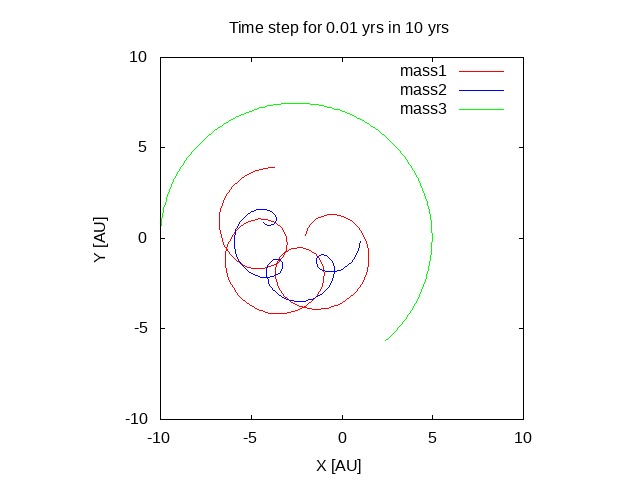
\includegraphics[scale=0.5]{pro1_result.png}
	\caption{Result of 3-body system in Python.} %圖片註解
	\label{fig.pro1a} %label 用這個就可以引用文章當中
\end{figure}

\begin{figure}[h]
    \centering
    \subfigure[fortran vs Python  in update pos/vel]{
        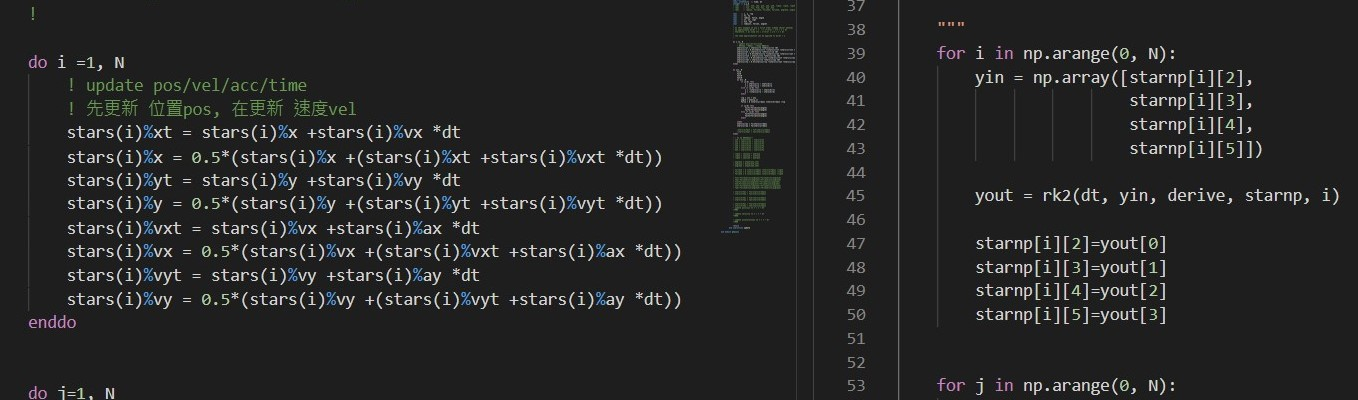
\includegraphics[scale=0.33]{pro1a_change.jpg}
        \label{fig.pro1a_ch}}
    \subfigure[fortran vs Python  in update acc]{
        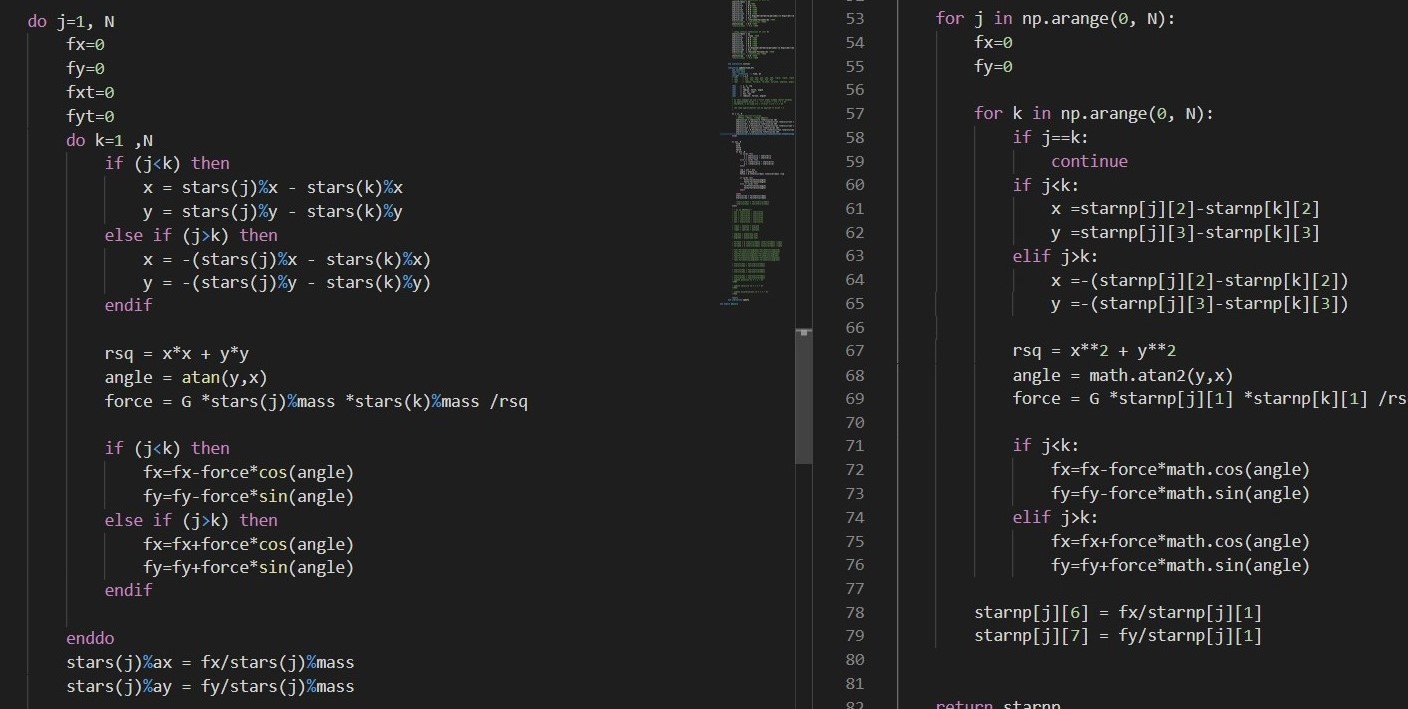
\includegraphics[scale=0.31]{pro1a_ac.jpg}
        \label{fig.pro1a_ac} }
    \caption{fortran vs Python}
    \label{fig.pro1a_}
\end{figure}

In this part, I use the same structure as the last lecture's assignment to code my python program. I try to use the generalized version, which can make binary system extend to simulate in n body system. In this program, time will mainly take on the second part(Fig.\ref{fig.pro1a_ac}.) in my update function in \emph{physics} file, because in this part the program need to calculate the distance between each two stars to measure the total force to act on every single star, the loop will take much time.\\

\textbf{1b.Compare the performance}\\

In conclusion, the performance of python used in \emph{numpy} package is more efficient than fortran.\\
I use \emph{timeit} package in python to calculate the time program run 5 times, the result is approximately 9~10[sec](Fig.\ref{fig.pro1b_py}.). In fortran, I use the command \emph{system\_clock()} to do measurement.(Note: \emph{system\_clock()} measure the time take by whole program, if only want to measure CPU time, can use the command \emph{cpu\_time()} ) The time fortran takes in 1 time is about 4.8[sec](Fig.\ref{fig.pro1b_for}.) in average.
\begin{figure}[h]
    \centering
    \subfigure[Time for python take 5 times]{
        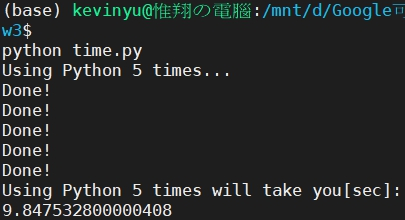
\includegraphics[scale=0.5]{pro1b_py.jpg}
        \label{fig.pro1b_py}
    }
    \subfigure[Time for fortran take 1 times]{
        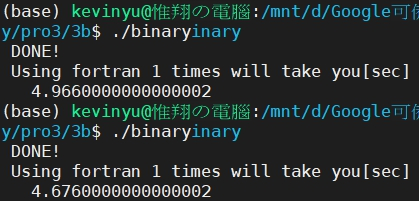
\includegraphics[scale=0.55]{pro1b_for.jpg}
        \label{fig.pro1b_for} 
    }
    \caption{Time spend by python vs fortran}
    \label{fig.pro1b}
\end{figure}

\underline{\textbf{Q2 : Gravitational Potential of 3-Body System}}\\
% %-------------------------------
In this part, I use the command called: \emph{contourf}, which is the instruction of package \emph{matplotlib.pyplot}.

About x \& y axis value, I Divide these axis by AU to make the axis more readable. The gravitational potential is also divided by AU, so the power of it come to $e13$.
The following are levels I chose to plot the equipotential contours.
$$ level1.\quad3.000\times10^{12} \qquad\ (white-gray\ blue) $$
$$ level2.\quad6.870\times10^{12} \quad (gray\ blue-light\ blue)  $$
$$ level3.\quad1.000\times10^{13} \ (light\ blue-middle\ blue) $$
$$ level4.\quad1.821\times10^{13} \ (middle\ blue-dark\ blue)$$
$$ level5.\quad3.000\times10^{13} \qquad\ \ (dark\ blue-white)$$
\begin{figure}[h]
    \centering 
	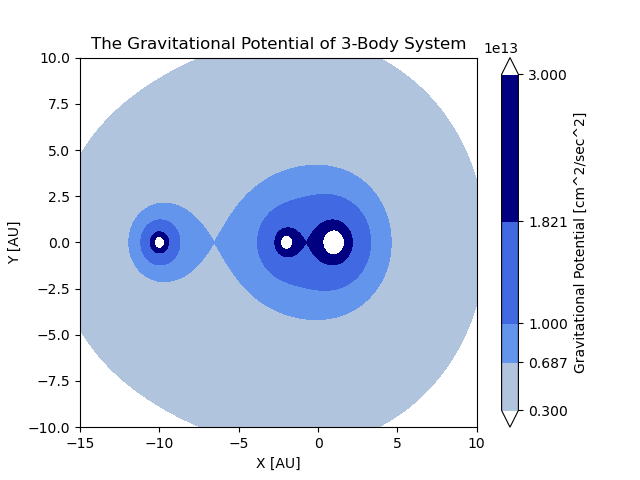
\includegraphics[scale=0.62]{Potential.png}
	\caption{Gravitational Potential of 3-Body System in log scale when time=0.} %圖片註解
	\label{fig.pro2} %label 用這個就可以引用文章當中
\end{figure}
% %-------------------------------

Special remark \textbf{level2 \& level3},
they all can imply there are points where have balanced gravitational force
\footnote{Lagrangian point:\href{https://en.wikipedia.org/wiki/Lagrange\_point}{https://en.wikipedia.org/wiki/Lagrange\_point}}
in this 3-body system.(Lagrangian point 2 which lies on the line between two objects.).

In Fig.\ref{fig.pro2}., we can see two Lagrangian points: One is implied by line2, $L_2$ is on the line between left star(x=-10[AU]) \& binary star in the right side. The other one is implied by line4, $L_2$ is inside the binary system.

\end{document}
% %-------------------------------
% \begin{figure}[h]
%     \centering 
% 	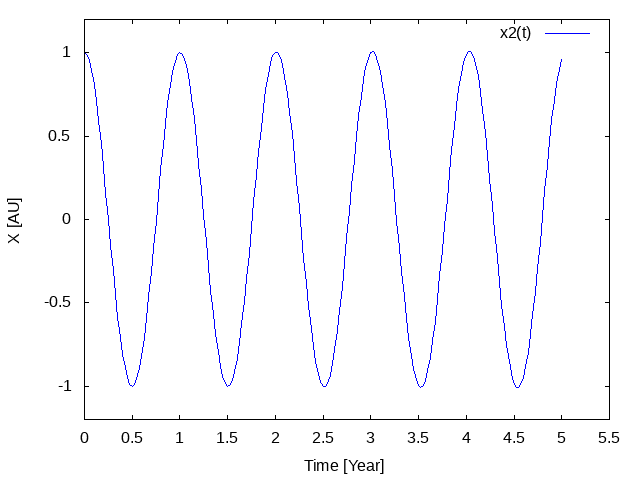
\includegraphics[scale=0.45]{pro1_x2.png}
% 	\caption{The trajectory of $m_1$ $m_2$ (when $m_2$ has a 1.25 factor of velocity).} %圖片註解
% 	\label{fig.pro1} %label 用這個就可以引用文章當中
% \end{figure}
% %-------------------------------

% %-------------------------------
% \begin{figure}[h]
%     \centering
%     \subfigure[dt=0.01yr]{
%         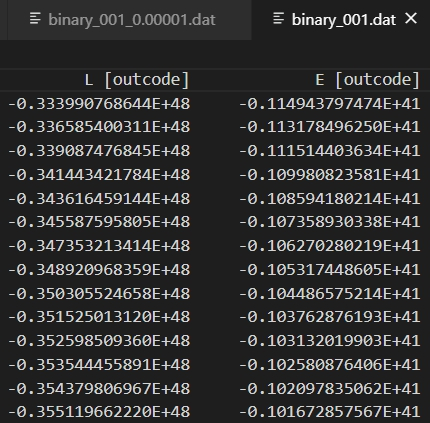
\includegraphics[scale=0.33]{01.jpg}
%         \label{01}
%     }
%     \subfigure[dt=0.001yr]{
%         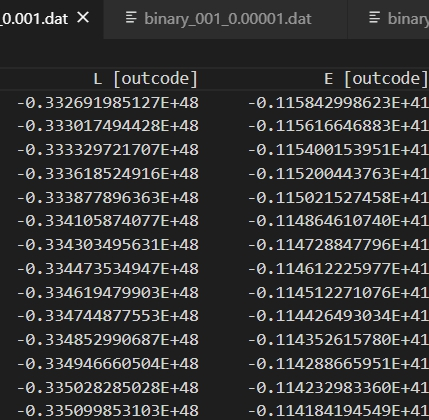
\includegraphics[scale=0.33]{001.jpg}
%         \label{001} 
%     }
%     \subfigure[dt=0.00001yr]{
%         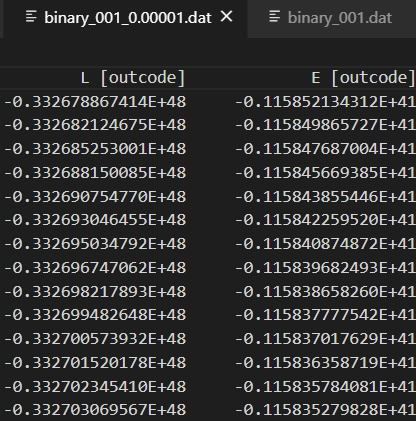
\includegraphics[scale=0.33]{00001.jpg}
%         \label{00001} 
%     }
%     \caption{L \& E in 0.01,0.001,0.00001 time step}
%     \label{fig:2c_dat}
% \end{figure}
% %-------------------------------